\chapter{Input and output}

%A number of years ago, Jeannette Wing published a terrific editorial with the title {\it Computational Thinking}, or in her own words, ``Ways to Think Like a Computer Scientist'' (see Communications of the ACM, March 2006).
%This 3-page article summarizes many of the problem-solving techniques you will discover while learning to program.
%Everyone interested in learning computer science beyond programming should read it.
%She defines the field this way:

%\index{computer science}

%\begin{quote}
%{\bf ``Computer science is the study of computation---what can be computed and how to compute it.''}
%\end{quote}

The programs we've looked at so far just display messages, which doesn't involve a lot of real computation.
This chapter will show you how to read input from the keyboard, use that input to calculate a result, and then format that result for output.


\subsection{The System class}
\label{sec:system}
\index{System class}
\index{class!System}
\index{object}

\java{System.out.println} can display the value of any type of variable.
You can even use \java{println} to print the value of \java{System.out}:

\begin{code}
System.out.println(System.out);
\end{code}

The result is:

\begin{stdout}
java.io.PrintStream@685d72cd
\end{stdout}

\index{address}

From this output we can see that
\java{System.out} is a \java{PrintStream}, which is defined in a
package called \java{java.io}.  A {\bf package} is a collection of
related classes; \java{java.io} contains classes related to ``I/O'',
which stands for input and output.

After the \java{@} sign is the
location of the object in memory, which is called its {\bf address}.
In this example the address is \java{685d72cd}, but if you run the same code you will likely get something different.
%You can think of the address as a unique identifier for the object.

\java{System.out} is an {\bf object}, which means that it is a value
that provides methods.  Specifically, \java{System.out} provides methods
for displaying data, including \java{print} and \java{println}.
Numbers with type \java{int} and \java{double} are not objects because
they provide no methods.  Strings are objects; we will see some of their
methods soon.

%When you call \java{System.out.println}, you are referring to the \java{out} variable declared in the \java{System} class.
%The \java{out} variable's type is \java{PrintStream}, which provides methods for ``printing'' data.
%Both \java{System} and \java{PrintStream} are written in Java, and later in the book we'll examine their source code.
%For now, you should understand that \java{System.out} is a \java{PrintStream} {\bf object}.
%Because Java is an {\em object-oriented} language, much of the library is organized around objects that perform specific actions.

The \java{System} class is defined in a file called {\tt System.java},
and {\tt PrintStream} is defined in {\tt PrintStream.java}.  These
files are part of the Java {\bf library}, which is an extensive collection
of classes you can use in your programs.

\begin{figure}[!h]
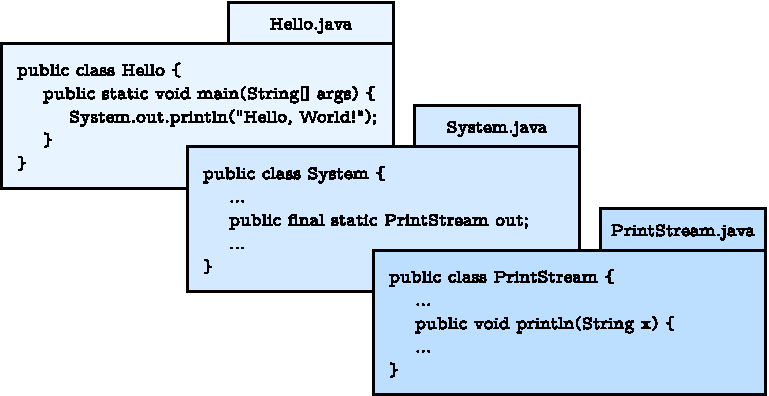
\includegraphics{system.pdf}
\caption{\java{System.out.println} refers to the \java{out} variable of the \java{System} class, which is a \java{PrintStream} that provides a method called \java{println}.}
\end{figure}

% ABD: there is no much new vocab in these sections, I want to reduce
% the number of new ideas

%\index{operating system}

%As with most software, Java programs run on top of an {\bf operating system} that manages the keyboard, the display, main memory, disk drives, printers, the network, and other hardware resources.
%Common examples of operating systems include Android, iOS, Linux, Mac OS~X, and Windows.
%When starting Java programs, the operating system directs \java{System.out} to the screen.

%\index{abstraction}

%Note the exact type of display doesn't matter, whether it's a 5-inch touch screen or 30-inch monitor.
%From the programmer's point of view, \java{System.out} simply provides the means for printing messages.
%Computer scientists often use {\bf abstraction} to deal with the complexity of software.
%The \java{System} class is a platform-independent abstraction of the operating system.
%The operating system itself is a layer of abstraction on top of computer hardware.

\subsection{The Scanner class}

\index{Scanner class}
\index{class!Scanner}
\index{byte}


%From the operating system's point of view, data from the keyboard arrives in a series of hardware control signals.
%The operating system translates these signals into a stream of {\bf bytes} (small integers), which in turn need to be translated into characters.

The \java{System} class also provides an object named \java{in}, which is an \java{InputStream} that provides methods for reading input from the keyboard.

\java{System.in} provides methods that perform simple operations, but they
are not easy to use.
Fortunately, Java provides other classes that make it easier to handle common tasks.

\index{class!utility}
\index{utility class}

For example, \java{Scanner} is a class that provides methods for
inputting words, numbers, and other types of data.  \java{Scanner}
is provided by \java{java.util}, which is a package that contains
classes so useful they are called {\bf utility classes}.

Before you can use \java{Scanner}, you have to import it like this:

\begin{code}
import java.util.Scanner;
\end{code}

This {\bf import statement} tells the compiler that when you say \java{Scanner}, you mean the one defined in {\tt java.util}.  This
is useful because there might be another class named \java{Scanner}
in another package.  Using an import statement makes your
code unambiguous.

Next you have
to create a \java{Scanner} object using the keyword \java{new}.
The following code declares a \java{Scanner} variable and then creates a \java{Scanner}:

\begin{code}
    Scanner in;
    in = new Scanner(System.in);
\end{code}

Although \java{Scanner} is not a function, the syntax is the same
as a function call.  We pass \java{System.in} as an
argument, which specifies that we are planning to input values from
the keyboard.

\index{initialize}

You can also declare the variable and initialize it at the same time:

\begin{code}
    Scanner in = new Scanner(System.in);
\end{code}

The new \java{Scanner} object provides a method called \java{nextLine} that reads a line of input from the keyboard and returns a String.
The following example reads two lines and repeats them back to the user.

\begin{code}
import java.util.Scanner;

public class Echo {

    public static void main(String[] args) {
        String line;
        Scanner in = new Scanner(System.in);

        System.out.print("Type something:");
        line = in.nextLine();
        System.out.println("You said: " + line);

        System.out.print("Type something else:");
        line = in.nextLine();
        System.out.println("You also said: " + line);
    }
}
\end{code}

If you omit the import statement and refer to \java{Scanner}, you will get a compiler error like ``cannot find symbol'', which means the compiler doesn't know what you mean by \java{Scanner}.

You might wonder why we can use the \java{System} class without importing
it.  \java{System} belongs to the \java{java.lang} package, which is
imported automatically.
According to the documentation, \java{java.lang} ``provides classes that are fundamental to the design of the Java programming language.''


\section{The structure of computer programs}

At this point, we have seen all of the elements that make up Java programs.
The following figure shows these organizational units.

\begin{figure}[!h]
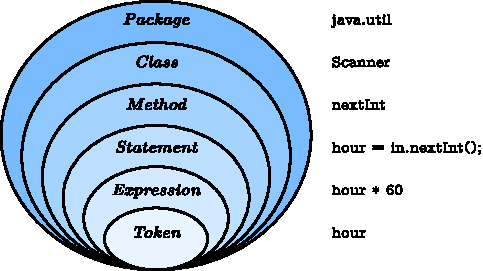
\includegraphics[width=4in]{package.pdf}
\caption{Elements of the Java language, from largest to smallest.}
\end{figure}

To review, a package is a collection of classes, which define methods.
Methods contains statements, some of which contain expressions.  Expression
are made up of tokens, which include variable names, numbers, operators,
keywords, and punctuation like braces and semi-colons.




\section{Inches to centimeters}

%An everyday problem that computers are great at solving is converting numbers from one unit into another.
Now let's see an example that's a little more useful.
Although most of the world has adopted the metric system for weights and measures, some countries are stuck with English units.
For example, when talking with friends in Europe about the weather, people in the United States may have to convert from Celsius to Fahrenheit and back.
Or you might want to convert your height in inches to centimeters.

%For the rest of the chapter, we will look at how to write programs that solve these types of problems.
%Specifically, each program will 1) prompt the user for input, 2) read input from the keyboard, 3) calculate a result, and 4) format the result for output.
%The focus will not only be on Java syntax and language features, but also on the {\em process} of solving the problem, documenting the code, and testing the solution.

We can write a program to help.  We can use a \java{Scanner} to 
input a measurement in inches, convert to centimeters, and then print
the results.

These lines declare the variables and create the \java{Scanner}:

% ABD: I am inclined not to include comments in most of the code
% examples because (1) I think it makes the code less cluttered and
% easier to read, and (2) they are often redundant with the text.

% I understand that it would be good to demonstrate good commenting
% style.  Despite this benefit, I think it's better to leave
% them out.  But I don't feel strongly about it.

\begin{code}
    int inch;  // the input
    double cm;  // the output
    Scanner in = new Scanner(System.in);
\end{code}

The first step is to prompt the user for the input.
We'll use \java{print} instead of \java{println} so they can enter the input on the same line.

\begin{code}
    // prompt the user and get the value
    System.out.print("How many inches? ");
    inch = in.nextInt();
\end{code}

Next we multiply the number of inches by 2.54, since that's how many centimeters there are per inch.
Finally we display the results on one line, but use two print statements since it's easier to read.

\begin{code}
    // convert and output the result
    cm = inch * 2.54;
    System.out.print(inch + " in = ");
    System.out.println(cm + " cm");
\end{code}

\index{magic number}

This code works, but it has a problem.  If another programmer reads
this code, they might wonder where 2.54 comes from.
Numbers like this that appear in an expression with no explanation are called {\bf magic numbers}.  For the benefit of other programmer (and yourself in the future), it is helpful to assign magic numbers to variables with informative names:

\begin{code}
    // convert and output the result
    final double cmPerInch = 2.54;
    cm = inch * cmPerInch;
    System.out.print(inch + " in = ");
    System.out.println(cm + " cm");
\end{code}

% ABD: if we postpone ``final'', we should remove it from this example.
% Or maybe this would be a good place to introduce it!



\subsection{Formatting output}

When printing floating-point numbers, Java automatically decides how many decimal places to display.

% ABD: What do you think of using the DrJava interpreter format to
% show the result of simple examples, as in the following?

\begin{code}
> System.out.print(7.0 / 3.0);
2.3333333333333335   note: 5 is a rounding error
\end{code}

\index{printf}

\java{System.out} provides a method called \java{printf}, where the ``f'' stands for ``formatted''.  The first argument of \java{printf} is a {\bf format string} that specifies how values should be displayed.
The following arguments are the values.
For example:

\begin{code}
    System.out.printf("Seven thirds = %.3f", 7.0 / 3.0);
    // prints 2.333
\end{code}

The format string contains ordinary text followed by a {\bf format specifier}, which is a special sequence that starts with a percent sign (\java{\%}).
The format specifier \java{\%.3f} indicates that the value should be displayed as floating-point with three decimal places.

Here's an example that contains two format specifiers:

\begin{code}
> inch = 100;
> cm = inch * cmPerInch;
> System.out.printf("%d in = %f cm\n", inch, cm);
100 in = 254.000000 cm  
\end{code}

The values are matched up with the format specifiers in order, so \java{inch}
is displayed as an integer (``d'' stands for ``decimal'') and
\java{cm} is displayed as a floating-point number.

The format string ends with a newline character (\java{\\n}) because \java{printf} does not append a newline like \java{println} does.

Learning \java{printf} is like learning a sub-language within Java.
There are many options, and the details can be overwhelming.
But here are some common uses, to give you an idea of how it works:

\begin{table}[!h]
\begin{tabular}{|l|l|l|}
\hline
{\tt \%d} & decimal integer & 12345 \\
\hline
{\tt \%,d} & decimal integer with comma separators & 12,345 \\
\hline
{\tt \%08d} & padded with zeros, at least 8 digits wide & 00012345 \\
\hline
{\tt \%f} & floating-point & 6.789000 \\
\hline
{\tt \%.2f} & floating-point {\em rounded} to 2 decimal places & 6.79 \\
\hline
\end{tabular}
\caption{Example format specifiers}
\end{table}

For more details, refer to the documentation of \java{java.util.Formatter}
of search the web for ``java formatting.''

As an exercise, see what happens if you try to display value with
type \java{int} using \java{\%f}.  And what happens if you display
a \java{float} using \java{\%d}?


\section{Centimeters to inches}
\label{sec:rounding}

Now suppose we have a measurement in centimeters and we want to
round it off to the nearest inch.  It is tempting to write:

\begin{code}
> inch = cm / centPerInch;
\end{code}

But the result is an error, something like, ``Bad types in
assignment: from double to int.''  The problem is that the value
on the right hand side is floating-point and the variable on the
left is an integer.


%How do we convert values in the other direction?
%Unfortunately, we can't just say \java{inch = cent / centPerInch;} because Java won't assign a \java{double} value to an \java{int} variable.
%We could change the declaration of \java{inch} to be a \java{double}, but there's another way.

%Java converts an \java{int} to a \java{double} automatically, since no information is lost in the process.
%On the other hand, going from \java{double} to \java{int} gets rid of the decimal places.
%Java doesn't perform this operation automatically in order to ensure that you are aware of the loss of the fractional part of the number.

\index{type cast}
\index{operator!cast}

The simplest way to convert a floating-point value to an integer is to use a {\bf type cast}, so called because it molds or ``casts'' a value from one shape to another.
The syntax for type casting is to put the name of the type in parentheses and use it as an operator.

\begin{code}
    double pi = 3.14159;
    int x = (int) pi;
\end{code}

\index{truncate}

The \java{(int)} operator has the effect of converting what follows into an integer.
In this example, \java{x} gets the value 3.
Converting to an integer always rounds down (toward zero), even if the fraction part is 0.999999.

Type casting takes precedence over arithmetic operations.

\begin{code}
    double pi = 3.14159;
    double x = (int) pi * 20.0;
\end{code}

In this example, the value of \java{pi} gets converted to an integer first, so the result is 60.0, not 62.

Keeping that in mind, here's how we can round a measurement in
centimeters to the nearest inch:

\begin{code}
    // convert and output the result
    inch = (int) (cm / centPerInch);
    System.out.printf("%f cm = %d in\n", cent, inch);
\end{code}

The parentheses after the cast operator require the division to
come before the type cast.


\subsection{Modulus operator}

Let's take the example one step further: suppose you have a measurement
in inches and you want to convert to feet and inches.
The goal is divide by 12 (the number of inches in a foot) and keep the remainder.

\index{modulus}
\index{operator!modulus}

We have already seen the division operator, \java{/}, which computes
the quotient of two numbers.  If the numbers are integers, it performs
floor division.
Java also provides the {\bf modulus} operator, \java{\%}, which
divides two numbers and computes the remainder.  Assuming that
\java{inch} is an integer, we can convert 76 inches to feet and inches like this:

\begin{code}
    int quotient = 76 / 12;   // division
    int remainder = 76 % 12;  // modulus
\end{code}

The first line yields 6.
The second line, which is pronounced ``76 mod 12'', yields 4.
So 76 inches is 6 feet, 4 inches.

The modulus operator is a percent sign ({\tt \%}), but you might find it helpful to think of it as a division sign ($\div$) rotated to the left.

\index{divisible}
\index{extract digits}

The modulus operator turns out to be surprisingly useful.  For
example, you can check whether one number is divisible by another: if
{\tt x \% y} is zero, then {\tt x} is divisible by {\tt y}.  You can
also use modulus to extract digits from a number: {\tt x \% 10} yields
the rightmost digit of {\tt x}.  Similarly, {\tt x \% 100} yields the
last two digits.  Also, many encryption algorithms are based on
modular arithmetic.


\section{Putting it all together}

At this point you know enough Java to write useful programs that solve everyday problems.
Here are the operations we've seen in this chapter:

\begin{itemize}

%% Chapter 1
%\item Write a class and main
%\item Display simple output
%\item Compile and run programs
%\item Correct syntax errors

%% Chapter 2
%\item Declare/assign variables
%\item Create named constants
%\item Perform basic arithmetic
%\item Compose multiple operations

%% Chapter 3
%\item Browse the Java library
\item Import Java library classes
\item Initialize a Scanner object
\item Get input from the keyboard
\item Read/write documentation
\item Format output with printf
\item Divide and mod integers

\end{itemize}

Now we can put them together in a complete program:

\begin{code}
import java.util.Scanner;

/**
 * Converts centimeters to feet and inches.
 */
public class Convert {
    public static void main(String[] args) {
        double cm;
        int feet, inches;
        final double centPerInch = 2.54;
        Scanner in = new Scanner(System.in);

        // prompt the user and get the value
        System.out.print("Exactly how many cm? ");
        cm = in.nextDouble();

        // convert and output the result
        inches = (int) (cm / centPerInch);
        feet = inches / 12;
        inches = inches % 12;
        System.out.printf("%.2f cm = %d ft, %d in\n",
                          cm, feet, inches);
    }
}
\end{code}

Notice:

\begin{itemize}

\item Although not required, all variables and constants are declared at the top of \java{main}.
This practice makes it easier to find their types later on and helps the reader know what data is involved in the algorithm.

\item Integer division and modulus often go together.
Notice how \java{inches} gets reassigned (which replaces its value) just before the \java{printf}.

\item When statements get long (generally wider than 80 characters), a common style convention is to break them across multiple lines.
The reader should never have to scroll horizontally.

\end{itemize}

%As an exercise, try running this code through Checkstyle.


\section{Reading documentation}
\label{sec:apidocs}

\index{documentation}

Now would be a good time to take a look at the documentation for \java{Scanner}.
You can find it in the Java library (see the link earlier in this chapter) or simply do a web search for ``java scanner.''
The latter method is more useful in the long run, especially as Oracle releases new versions of Java.
Either way, you should get something like this:

\begin{figure}[!h]
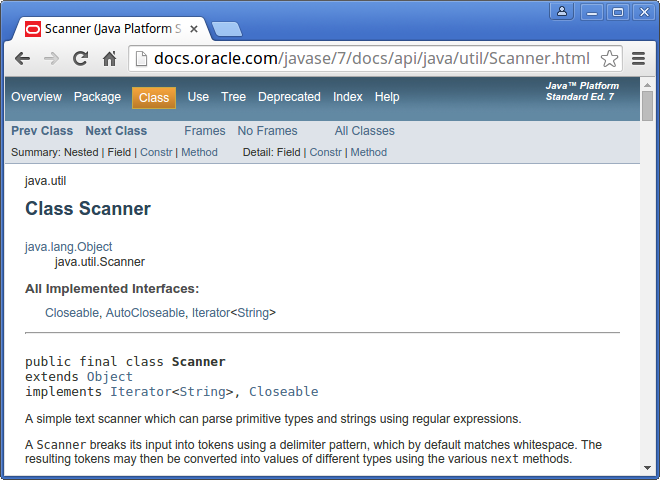
\includegraphics[width=\textwidth]{scanner.png}
\caption{Screenshot of the documentation for \java{Scanner} on Oracle's website.}
\end{figure}

Scroll down to the ``Method Summary'' section.
As you can see, the \java{Scanner} class provides quite a few methods.
In this chapter we'll focus on the ``next'' methods.
For example, click on the link for \java{nextInt}.

\begin{stdout}
public int nextInt()

Scans the next token of the input as an int.
\end{stdout}

\index{prototype}

The first line is the method's {\bf prototype}, which specifies the name of the method and its return type.
In this example, \java{nextInt} returns an \java{int}.
The next line describes what the method does.
The subsequent lines (not shown) explain the parameters and return values.
Explanations are often redundant, but the documentation is supposed to fit this standard format.
%The last line describes the exceptions this method might throw.

It might take some time to get comfortable reading this kind of information, but it's well worth the effort.
Knowing what methods a class provides helps you avoid reinventing the wheel.
Whenever you learn about a new class, you should take a quick look at its documentation.
On that note, take a few minutes to review the documentation for \java{System} and \java{String}.


\section{Writing documentation}

\index{Javadoc}

A nice feature of the Java language is the ability to write documentation at the same time you are writing the source code.
That way, the documentation stays in sync with the classes and methods themselves.
In fact, the HTML pages you browsed in the previous section were automatically generated using a tool called {\bf Javadoc}.
This tool is part of the standard JDK, and you can run it directly from DrJava by pressing the {\tt Javadoc} button on the toolbar.

\index{comments!documentation}
\index{documentation comments}

Javadoc parses your source files for {\bf documentation comments} and extracts other relevant information about your class and method definitions.
Given the prevalence of this tool, people sometimes refer to documentation as ``Javadoc comments.''
In contrast to inline comments that begin with {\tt //}, documentation comments begin with {\tt /**} (two stars) and end with {\tt */} (one star).
Anything in between these two tokens becomes part of the documentation.
As a rule of thumb, you should document every class and every method.

\begin{code}
/**
 * Example program that demonstrates print vs println.
 */
public class Goodbye {

    /**
     * Application entry point; simply prints a greeting.
     */
    public static void main(String[] args) {
        System.out.print("Goodbye, ");  // note the space
        System.out.println("cruel world");
    }

}
\end{code}

This example has perhaps too many comments, since all the program does is print a message.
But it illustrates the differences between inline and documentation comments:

\begin{itemize}
\item Inline comments tend to be short phrases that help explain complex parts of a method.
Documentation comments are typically complete sentences that begin with a capital letter and end with a period.

\item Documentation comments often span multiple lines.
By convention, each line begins with a {\tt *} that is aligned vertically with the start and end of the comment.

\item Some development environments (e.g., Eclipse and NetBeans) automatically display documentation comments when you hover your mouse over the name of a class or method.

\end{itemize}

Writing documentation and inline comments is essential for making source code readable.
As we discussed in the last chapter, people spend the majority of their development time understanding and modifying existing code.
You should not only write good comments for others, but for yourself as well.
When you haven't looked at your own code for a while, it takes a long time to remember how it works (or what you were trying to do) if there's no comments.


\section{Command-line testing}

%You really should review the advice in Section~\ref{sec:examples}, now that you've written some more substantial programs.
It's more effective to program and debug your code little by little than to attempt writing everything at once.
And once you've completed programming an algorithm, it's important to test that it works correctly on a variety of inputs.

Throughout the book, we will illustrate techniques for testing your programs.
Most if not all testing is based on a simple idea: does the program do what we expect it to do?
For simple programs, it's not difficult to run them several times and see what happens.
But at some point, you will get tired of typing the same test cases over and over.

We can automate the process of entering input and comparing {\em expected output} with {\em actual output} using the command-line.
The basic idea is to store the test cases in plain text files and trick Java into thinking they are coming from the keyboard.
Here are step by step instructions.

\begin{enumerate}

\item Make sure you can compile and run the {\tt Convert.java} example in the previous section.
%You can also download a copy from \url{http://thinkjava.org/}.

\item In the same directory as {\tt Convert.java}, create a plain text file named {\tt test.in} (``in'' is for input).
Enter the following line and save the file.

\begin{stdout}
193.04
\end{stdout}

\item Create a second plain text file named {\tt test.exp} (``exp'' is for expected).
Enter the following line and save the file.

\begin{stdout}
193.04 cm = 6 ft, 4 in
\end{stdout}

\item Open a command-line, and change to the directory with these files.
Run the following command to test the program.

\begin{stdout}
java Convert < test.in > test.out
\end{stdout}

\end{enumerate}

On the command-line, \java{<} and \java{>} are {\bf redirection operators}.
The first one redirects the contents of {\tt test.in} to \java{System.in}, as if it were entered from the keyboard.
The second one redirects the contents of \java{System.out} to a new file {\tt test.out}, much like a screen capture.
In other words, the {\tt test.out} file contains the output of your program.

By the way, it's perfectly okay to compile your programs in DrJava (or some other environment) and run them from the command-line.
Knowing both techniques allows you to use the right tool for the job.

At this point, we just need to compare the contents {\tt test.out} with {\tt test.exp}.
If the files are the same, then the program outputted what we expected it to output.
If not, then we found a bug, and we can use the output to begin debugging our program.
Fortunately, there's a simple way to compare files on the command-line:

\begin{stdout}
diff test.exp test.out
\end{stdout}

The {\tt diff} utility summarizes the differences between two files.
If there are no differences, then it prints nothing, which in our case is what we want.
If the expected output differs from the actual output, then we need to debug our program.
Or in some cases, we need to debug our test cases.
There's always a chance we have a correct program and a typo in the expected output.

% ABD: Since I killed the previous reference to abstraction, I am inclined
% to kill this one too.  The problem in both places is that it pulls the
% focus off topic.

%Redirecting a program's input and output is an example of how computer scientists use abstraction.
%Notice that \java{System.in} is not called \java{Keyboard}, and \java{System.out} is not called \java{Display}.
%In practice, these objects could be text files, network connections, microphones and speakers, or some other byte streams.
%What's great is that doesn't change anything about how you write the code.
